\documentclass[a4paper,11pt]{article}
\usepackage{amsmath}
\usepackage{amssymb}
\usepackage[polish]{babel}
\usepackage{polski}
\usepackage[utf8]{inputenc}
\usepackage{indentfirst}
\usepackage{geometry}
\usepackage{array}
\usepackage[pdftex]{color,graphicx}
\usepackage{subfigure}
\usepackage{afterpage}
\usepackage{setspace}
\usepackage{color}
\usepackage{wrapfig}
\usepackage{listings}
\usepackage{datetime}

\renewcommand{\onehalfspacing}{\setstretch{1.6}}

\geometry{tmargin=2.5cm,bmargin=2.5cm,lmargin=2.5cm,rmargin=2.5cm}
\setlength{\parindent}{1cm}
\setlength{\parskip}{0mm}

\newenvironment{lista}{
\begin{itemize}
  \setlength{\itemsep}{1pt}
  \setlength{\parskip}{0pt}
  \setlength{\parsep}{0pt}
}{\end{itemize}}

\newcommand{\linia}{\rule{\linewidth}{0.4mm}}

\definecolor{lbcolor}{rgb}{0.95,0.95,0.95}
\lstset{
    backgroundcolor=\color{lbcolor},
    tabsize=4,
  language=C++,
  captionpos=b,
  tabsize=3,
  frame=lines,
  numbers=left,
  numberstyle=\tiny,
  numbersep=5pt,
  breaklines=true,
  showstringspaces=false,
  basicstyle=\footnotesize,
  identifierstyle=\color{magenta},
  keywordstyle=\color[rgb]{0,0,1},
  commentstyle=\color{Darkgreen},
  stringstyle=\color{red}
  }

\begin{document}

\noindent
\begin{tabular}{|c|p{11cm}|c|} \hline 
Z2 & Przemysław Kleszcz, Krzysztof Tatar & \ddmmyyyydate\today \tabularnewline
\hline 
\end{tabular}


\section*{Zadanie 4 - Liczby pierwsze - OpenMP}

Celem zadania było napisanie programu, który testuje podane duże liczby pierwsze. Do poprawnego działania programu należy podać dwa argumenty wejściowe są to \emph{n -liczba wątków} i \emph{primes - ścieżka do pliku z liczbami pierwszym}. Poniżej zaprezentowano główną funkcje programu odpowiedzialną za zrównoleglanie obliczeń.


\begin{lstlisting}
int prime_number(string tnumber, int numOfThreads)
{
	int prime = 1;
	long long j;

	long long number = atoll(tnumber.c_str());
	bool flag = false;

#pragma omp parallel for shared(number, prime, flag) num_threads(numOfThreads) private(j) schedule(guided, 1)
	for (j = 2; j < number; j++)
	{
		if (flag)
			continue;

		if (number % j == 0)
		{
			prime = 0;
			flag = true;
		}
	}

	return prime;
}
\end{lstlisting}



Powyższy program sprawdza czy liczba jest pierwszą czy nie jest liczbą pierwszą. Do zrównoleglenia głównej pętli for została użyta dyrektywa biblioteki OpenMP.
Zrównoleglenie głównej pętli for: 
\begin{lstlisting}
#pragma omp parallel for
\end{lstlisting}
Wyraz omp jest słowem kluczowym OpenMP. Dyrektywa parallel, wskazuje kompilatorowi obszar kodu, który będzie zrównoleglony. Kolejna dyrektywa - for - informuje kompilator, że zrównoleglana będzie pętla typu for.
Określnie które zmienne będą wspólne shared, a które prywatne private:
\begin{lstlisting}
shared(number, prime, flag)
private(j)
\end{lstlisting}
Zmienne wspólne są dostępne dla każdego wątku, natomiast do danej zmiennej prywatnej ma dostęp tylko jeden określony wątek. W naszym programie zmienną prywatną jest j - licznik pętli, a zmiennymi wspólnymi number, prime, flag.
\newline
\newline
Dyrektywa schedule: 
\begin{lstlisting}
schedule(guided, 1)
\end{lstlisting}
Za pomocą polecenia schedule możemy kontrolować sposób w jaki OpenMP przydziela iteracje dostępnym wątkom. Parametr guided powoduje przypisanie do każdego wąktu odpowiednio dużego fragmentu następujących po sobie iteracji. Rozmiar fragmentu zmniejsza się wykładniczo, wraz z każdym pomyślnym przypisaniem, do minimalnego rozmiaru zdefiniowanego w parametrze „chunk”. Parametr „chunk” jest ustawiony na 1, oznacza to że rozmiar każdego z początkowych zbiorów jest opisany wyrażeniem: \begin{center}liczba\_nieprzydzielonych\_iteracji/liczba\_wątków
\end{center}
Dyrektywa num\_threads: 
\begin{lstlisting}
num_threads(numOfThreads)
\end{lstlisting}
Za pomocą dyrektywy num\_threads określa się ile wątków ma być użytych do zrównoleglenia pętli for.



\begin{figure}[!ht]
	\centering
 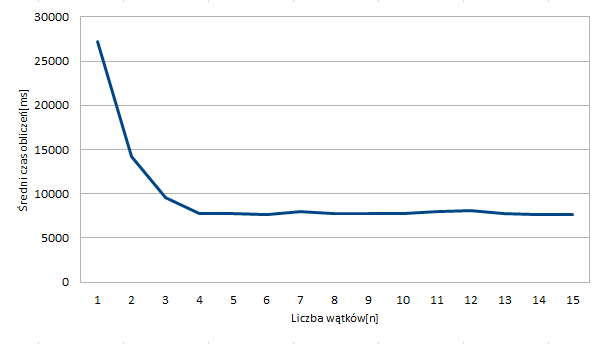
\includegraphics[width=0.7\textwidth]{1.png}
  \caption{Wykres średniego czasu obliczeń}
\end{figure}

Z powyższego rysunku można wywnioskować, że średni czas obliczeń dynamicznie malał dla pierwszych 4 wątków. Następnie dla kolejnych wątków średni czas jest ustabilizowany.
Poniższy rysunek jest dobrym przykładem opisanego zjawiska.


\begin{figure}[ht]
	\centering
  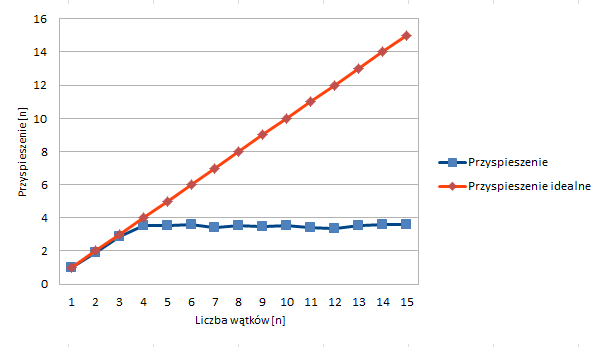
\includegraphics[width=0.7\textwidth]{2.png}
  \caption{Wykres przyspieszenia}
\end{figure}

Powyższe zadanie zostało zrównoleglone dzięki bibliotece OpenMP. Dzięki zastosowaniu dyrektyw biblioteki udało się uzyskać czterokrotne przyspieszenie dla 4 wątków. Dla kolejnych 11 wątków, w tym przykładzie nie wpłynęły znacząco na wydajność.

\end{document}
